\documentclass[a4paper]{article}

\usepackage[english]{babel}
\usepackage[utf8]{inputenc}
\usepackage{amsmath}
\usepackage{graphicx}
\usepackage{listings}
\usepackage{hyperref}
\hypersetup{
    colorlinks=true,
    linkcolor=blue,
    filecolor=magenta,      
    urlcolor=cyan,
}
\usepackage[colorinlistoftodos]{todonotes}

\title{Multi Agent Systems Report 1}

\author{Andrea Scorza, Diego Staphorst, Erik Lokhorst, Ingmar van der Geest}

\date{\today}

\begin{document}
\maketitle

\begin{abstract}
This is the first report for the negotiation agent project of Multi Agent Systems at Utrecht University. In the report the pareto efficient frontier is calculated for a single negotiation and two different negotiations with various agents are analysed. 
\end{abstract}

\section{Computing the pareto efficient frontier}
\begin{figure}[h!]
\centering
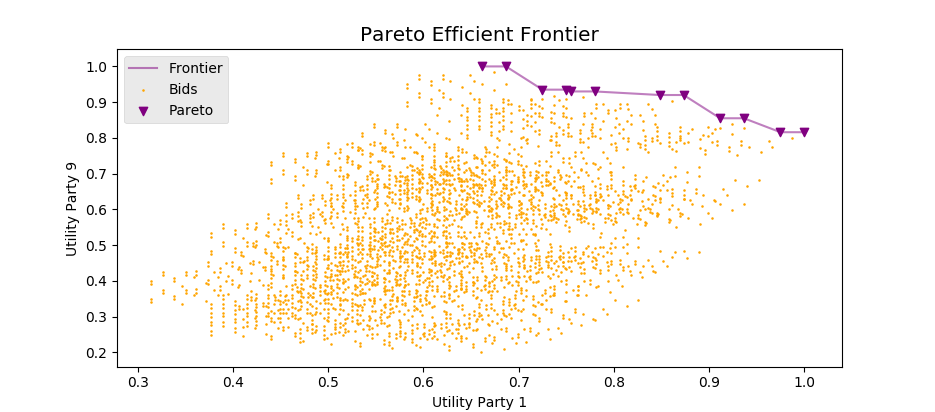
\includegraphics[width=125mm]{pareto_efficient.png}
\caption{\label{fig:pareto_figure} Pareto efficient frontier including the bids generated with matplotlib in python 3.7. We used the preferences of party 1 and party 9}  
\end{figure}
To visualize the pareto efficient frontier, we manually calculated utility values for each preference in Excel. In Python we were able to manipulate the data so, to get all the possible bids and with \href{https://sirinnes.wordpress.com/2013/04/25/pareto-frontier-graphic-via-python/}{Pareto frontier graphic via python} we were able to visualize the bids and Pareto Frontier.
\newpage
\section{Analysis of negotiations between various agents}

\subsection{Single negotiation between two simple agents}

The single negotiation lasted 17 rounds and ended with an agreement where $u(a1) = 0.777$ and $u(a2) = 0.510$. The strategy of both agents is to bid randomly until an agreement is reached, no optimisation of utility takes place (Figure \ref{fig:simplevssimple}). There is no pareto optimal outcome reached (distance to pareto = 0.199), if this would happen in this scenario it would be purely coincidental. See

\begin{figure}[h!]
\centering
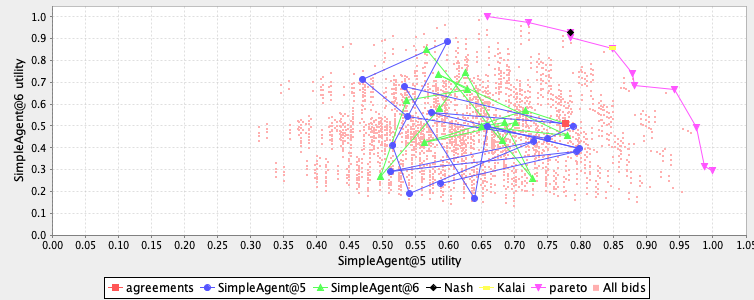
\includegraphics[width=125mm]{simplevssimple.png}
\caption{\label{fig:simplevssimple} Results graph of the negotiation between two simple agents in Genius.}  
\end{figure}

\subsection{Single negotiation between Boulware agent and Conceder agent}

The single negotiation lasted 83 rounds and ended with an agreement where $u(b) = 0.975$ and $u(c) = 0.495$. The strategy of the boulware agent is to bid its maximum utility (u=1) up until the last rounds, where it slowly starts to concede. The strategy of the conceder agent is to begin bidding its maximum utility (u=1) and in subsequent rounds lower its utility until an agreement is reached (Figure \ref{fig:boulvsconcede}). A pareto optimal outcome is reached (distance to pareto = 0.000). In different negotiations with different preference profiles a pareto optimal outcome was also reached. The Boulware agent performs very well against the conceder agent because the conceder will keep lowering its utility until it finds an agreement, at the same time the Boulware agent can simply stick with its near-optimal utility. 

\begin{figure}[h!]
\centering
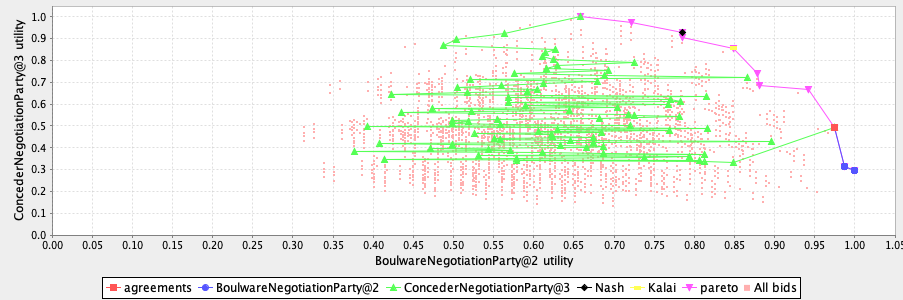
\includegraphics[width=125mm]{boulvsconcede.png}
\caption{\label{fig:boulvsconcede} Results graph of the negotiation between the Boulware agent vs the Conceder agent in Genius.}  
\end{figure}

\end{document}